\documentclass[12pt,a4paper]{report}

%Set language
\usepackage[english]{babel}

% To import and adjust images
\usepackage{graphicx}
\usepackage[export]{adjustbox}
\usepackage[center]{caption}
\usepackage{subcaption}

% Path relative to the .tex file containing the \includegraphics command
\graphicspath{ {./images/} }  

% To change the ToC title
\addto\captionsenglish{ \renewcommand {\contentsname} {Table of contents}}

\title{SafeStreets - RASD \\ \large version 1.0}
\author{Frangi Alberto, Fucci Tiziano}
\date{A.Y. 2019/2020}
\begin{document}
\maketitle

% Command to hide subsections in the index
\setcounter{tocdepth}{1}

% Index
\tableofcontents
\chapter{Introduction}
	\section{Purpose}
SafeStreets is a crowd-sourced application that intends to provide users with the possibility to notify authorities when traffic violations occur, and in particular parking violations, such as vehicles parked in the middle of bike lanes or in places reserved for people with disabilities, double parking, and so on. The application allows users to send pictures of violations, including their date, time, and position, to authorities.
 
SafeStreets stores the information provided by users, completing it with suitable meta-data. In particular, when it receives a picture, it runs an algorithm to read the license plate (one can also think of mechanisms with which the user can help with the recognition), and stores the retrieved information with theviolation, including also the type of the violation (input by the user) and the name of the street where the violation occurred (which can be retrieved from the geographical position of the violation). 

The application allows both end users and authorities to mine the information that has been received, for example by highlighting the streets (or the areas) with the highest frequency of violations, or the vehicles that commit the most violations. 

Moreover, if the municipality offers a service that allows users to retrieve the information about the accidents that occur on the territory of the municipality, SafeStrees can cross this information with its own data to identify potentially unsafe areas, and suggest possible interventions (e.g., add a barrier between the bike lane and the part of the road for motorized vehicles to prevent unsafe parking).


	\section{Scope}
	\subsection{General description}
Safestreet is an application to be used both from civilians (users) and authorities, in order to help the latter and reduce traffic violations. Registered authorities can automatically receive reports made by users, so the service acts as an intermediary. Reports are made of a picture of the violation and some... 
	%(to be reviewed and completed)
	\subsection{Goals}
	The following list describes the goals from the S2B perspective:
	
	% Dot list 
	\begin{itemize}
		\item \textbf{G1}: The application must allow users to notify traffic violations, providing  the type of violation and a picture of the vehicle.
	% Il resto se lo trova da solo
	  	\item \textbf{G2}: The application must allow authorities to retrieve the reports made by all the users at any moment.
		% \item \textbf{G3}: The application must read correctly the license plates from the pictures attached to reports. --assumption?
		\item \textbf{G3}: The application must be able to detect the streets and the vehicles with the highest frequency of violations.
		\item \textbf{G4}: The application must be able to identify potentially unsafe areas and suggest possible interventions.
		\item \textbf{G5}: The application must not show one user's reports to other users.
		\item \textbf{G6}: The application must allow every user to see all of his reports and their status.
	\end{itemize}

	\section{Definitions, acronyms, abbreviations}
		\subsection{Definitions}
		\begin{itemize}
		\item \textbf{User}: a civilian customer that can use the application to:
			\begin{itemize}
			\item notify authorities of some violation;
			\item check which are the most dangerous (i.e. with the most violations) streets;
			\item check which are the vehicles that committed the most violations.
			\end{itemize}
		\item \textbf{Authority}: a member of the local police who has access to reports made by users.
		\item \textbf{Report}: a message consisting of:
			\begin{itemize}
			\item a picture showing the car in order to show the occurring violation;
			\item date and time of the picture;
			\item GPS position of the place where the violation occurred;
			\item the street where the violation occurred (automatically retrieved from the geographical position);
			\item the type of the violation (input by the user)
			\end{itemize}
		\item \textbf{Violation}: a situation that, according to the user who sent the report, is a violation of the traffic laws.
		\item \textbf{Intervention}: a brief text suggesting a possible solution in order to improve safety and discourage future violations.
		\end{itemize}
		\subsection{Acronyms}
			\begin{itemize}
			\item \textbf{API}: \emph{Application Programming Interface.}
			\item \textbf{GPS}: \emph{Global Positioning System.}
			\item \textbf{UI}: \emph{User Interface.}		
			\item \textbf{S2B}: \emph{Software-to-be.}	
			\end{itemize}
		\subsection{Abbreviations}
% To be written

	\section{Revision history}
% To be written

	\section{Reference documents}
	\begin{itemize}
	\item {Specification document}: ``SafeStreets Mandatory Project Assignment''
	%to be completed
	\end{itemize}

	\section{Document structure}
	\begin{itemize}
	\item \textbf{Chapter 1} is an introduction: it presents the document and the S2B with its scope and goals. It also helps the reader to understand, by giving the necessary definitions and explaining acronyms and abbreviations. 
	\item \textbf{Chapter 2} is a summary description of all the project and how the main parts work. %Non so, ti va bene? i
	\item \textbf{Chapter 3} is the core of the document...
	\item \textbf{Chapter 4} contains the Alloy model of critical aspects that require special attention. Here it is shown how the project has been modeled and a proof of the model consistency is provided. Moreover, examples of some of the generated world are shown.
	\item \textbf{Chapter 5} is meant to show how work was divided between the two components of the group and how much time was spent.
	\item \textbf{Chapter 6} contains the list of references...
	\end{itemize}

% End of first chapter

\chapter{Overall description}
	\section{Product perspective}
		%missing introduction
		Safe Streets want to be a mediator between authorities and citizen, allowing the last ones to report traffic violations, see
		in which zone have the highest number of violations, and the recap of all the previous reports and their state
		(seen, approved, rejected, in queue). In order to be able to report various violations an user has to be in first place in a
		territory covered by any authorities who had signed up to Safe Streets, and has to sign up compiling a form, choosing a
		nickname, unique for each user, and a mail. Any authority has to verify its identity using the institutional email 
		%state case registration
		The system to avoid spamming of request pending reports will be in a priority queue based 
		on a reliability index associated to each user and hidden to both side of communication (is an information used only by 
		the system for the priority queue). If the authorities sanction a violation reported the user 
		will receive a notification by Safe Streets to inform him the success (or failure) of his report. 
		%inserire immagine diagramma come funziona report
	\section{Product functions}
		In the following section the most important product functions of the system are reported.
		Safe Streets offers the possibility to its users to report traffic violations, check the status of the previous reports and see 
		a map that indicates the areas with the highest number of report verified.
		\subsection{Report}
			To report a violation a user had to take a picture of the possible violation with the plate visible, choose what type of
			violation it is from various possible category and sending the position
		\subsection{Status}
			This functionality allows user to see a recap of all the reports they have made. The information that will be displayed
			are: Date and time, place, type of violation and status. The last one can be:
			\begin{itemize}
				\item \textbf{In queue:}
					In this status the report is waiting to be analyzed by an authority. The report's priority is based on
					the user who created it. All the user at the moment of registration has a standard value that based on
					how Safe Street is used can increase or decrease. Some important factors are, for example, 
					how many report a user sent has been rejected, how many report a user send in one time can decrease
					the priority, but a wisely use of the system can increase it, like a streak of approved reports.
				\item \textbf{Processing:}
					In this status the authorities has seen the report and are considering the violation and if it is a real
					violation.
				\item \textbf{Approved:}
					The report has been seen by authorities and the violation has been recognized and sanctioned 
				\item \textbf{Rejected:}
					The report has been seen by authorities and the violation hasn't been recognized.
			\end{itemize}
		\subsection{Map}
			This function allows the user to open the map and see the "level of violations" of the different areas. These "levels" are
			based on how many reports have been approved in that area, higher the level, higher the number of violation.
			There are 4 levels, are indicated with different color, from green (level 0) to red (level 3).
			
	\section{User characteristics}
		The actors of the application are the following:
		\begin{itemize}
			\item \textbf{User:}
				a person who has registered to SafeStreets, he doesn't need any particular skill to use the system, 
				he is just supposed to have a smartphone (or tablet) with a functioning camera, an internet connection and
				that his phone can send his current position. The user can send a report to notify the authorities various traffic
				violation, he can view a map that highlight the streets with an higher number of reports. To do a report is sufficient
				take a photo of the license plate, the violation's type and the system retrieves in autonomous the current position
				of the user.
			\item \textbf{Authority:}
				An agent of the local police of a municipality using SafeStreets, that has access to all the reports made in his municipality. The authority can visualize the available reports and valuate them, that is telling if the violation reported by the user stands or it is not a proper violation. After seeing a report, the authority changes its status to Approved or Rejected.
		\end{itemize}
	\section{Assumptions, dependencies and constraints}
		\begin{itemize}
			\item When the user send the report is in the same place of the violation.
			\item If an user can send a report the local municipality had joined Safe Streets.
		\end{itemize}
% End of second chapter

\chapter{Specific Requirments}
	\section{External interface requirments}
		\subsection{User interfaces}
		In this section some screenshots from the user interface are shown. 
		\begin{figure}[h]
		\begin{subfigure}{0.5\textwidth}
			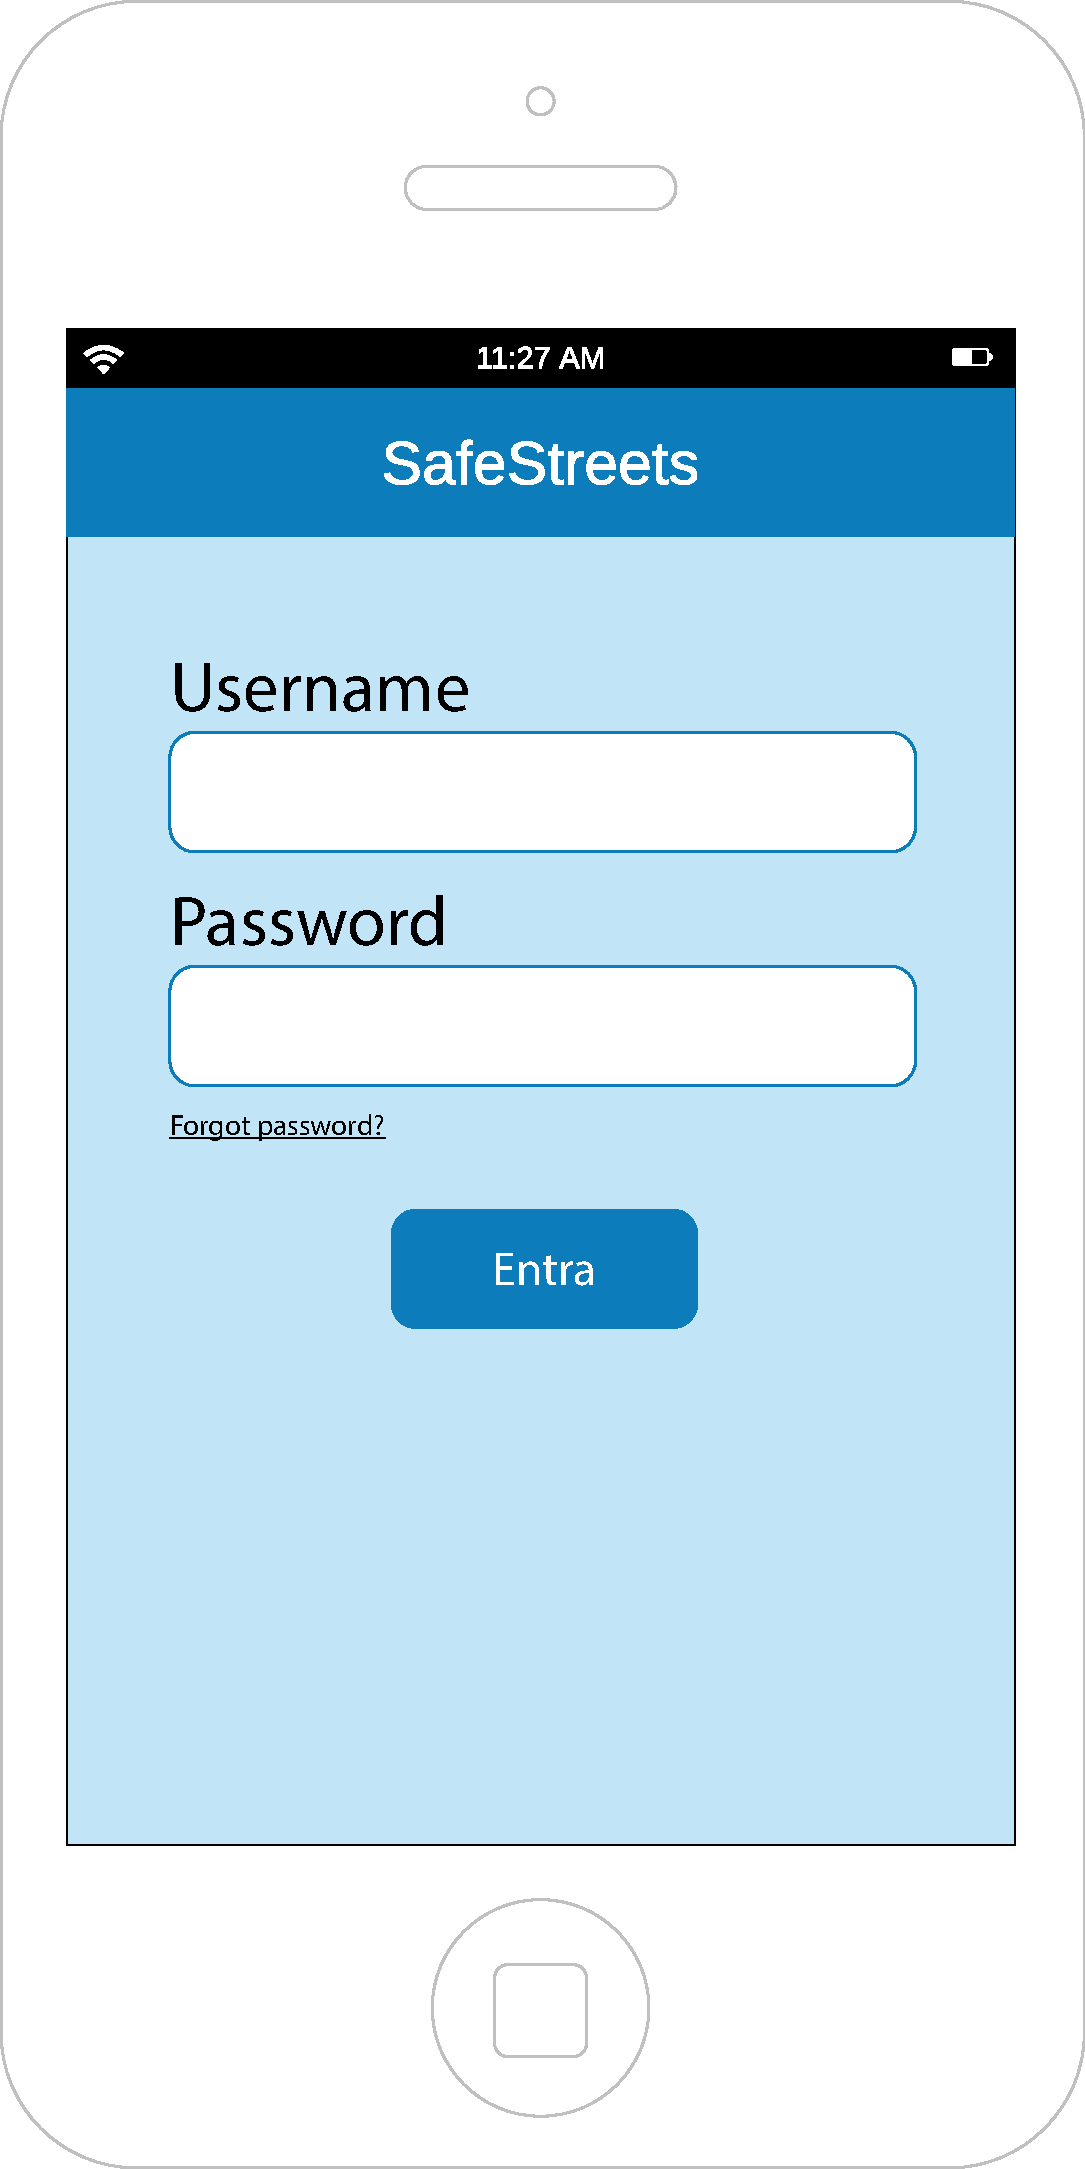
\includegraphics[scale=0.25, center]{Login}
			\caption{Login}
			\label{Login}
		\end{subfigure}
		\begin{subfigure}{0.5\textwidth}
			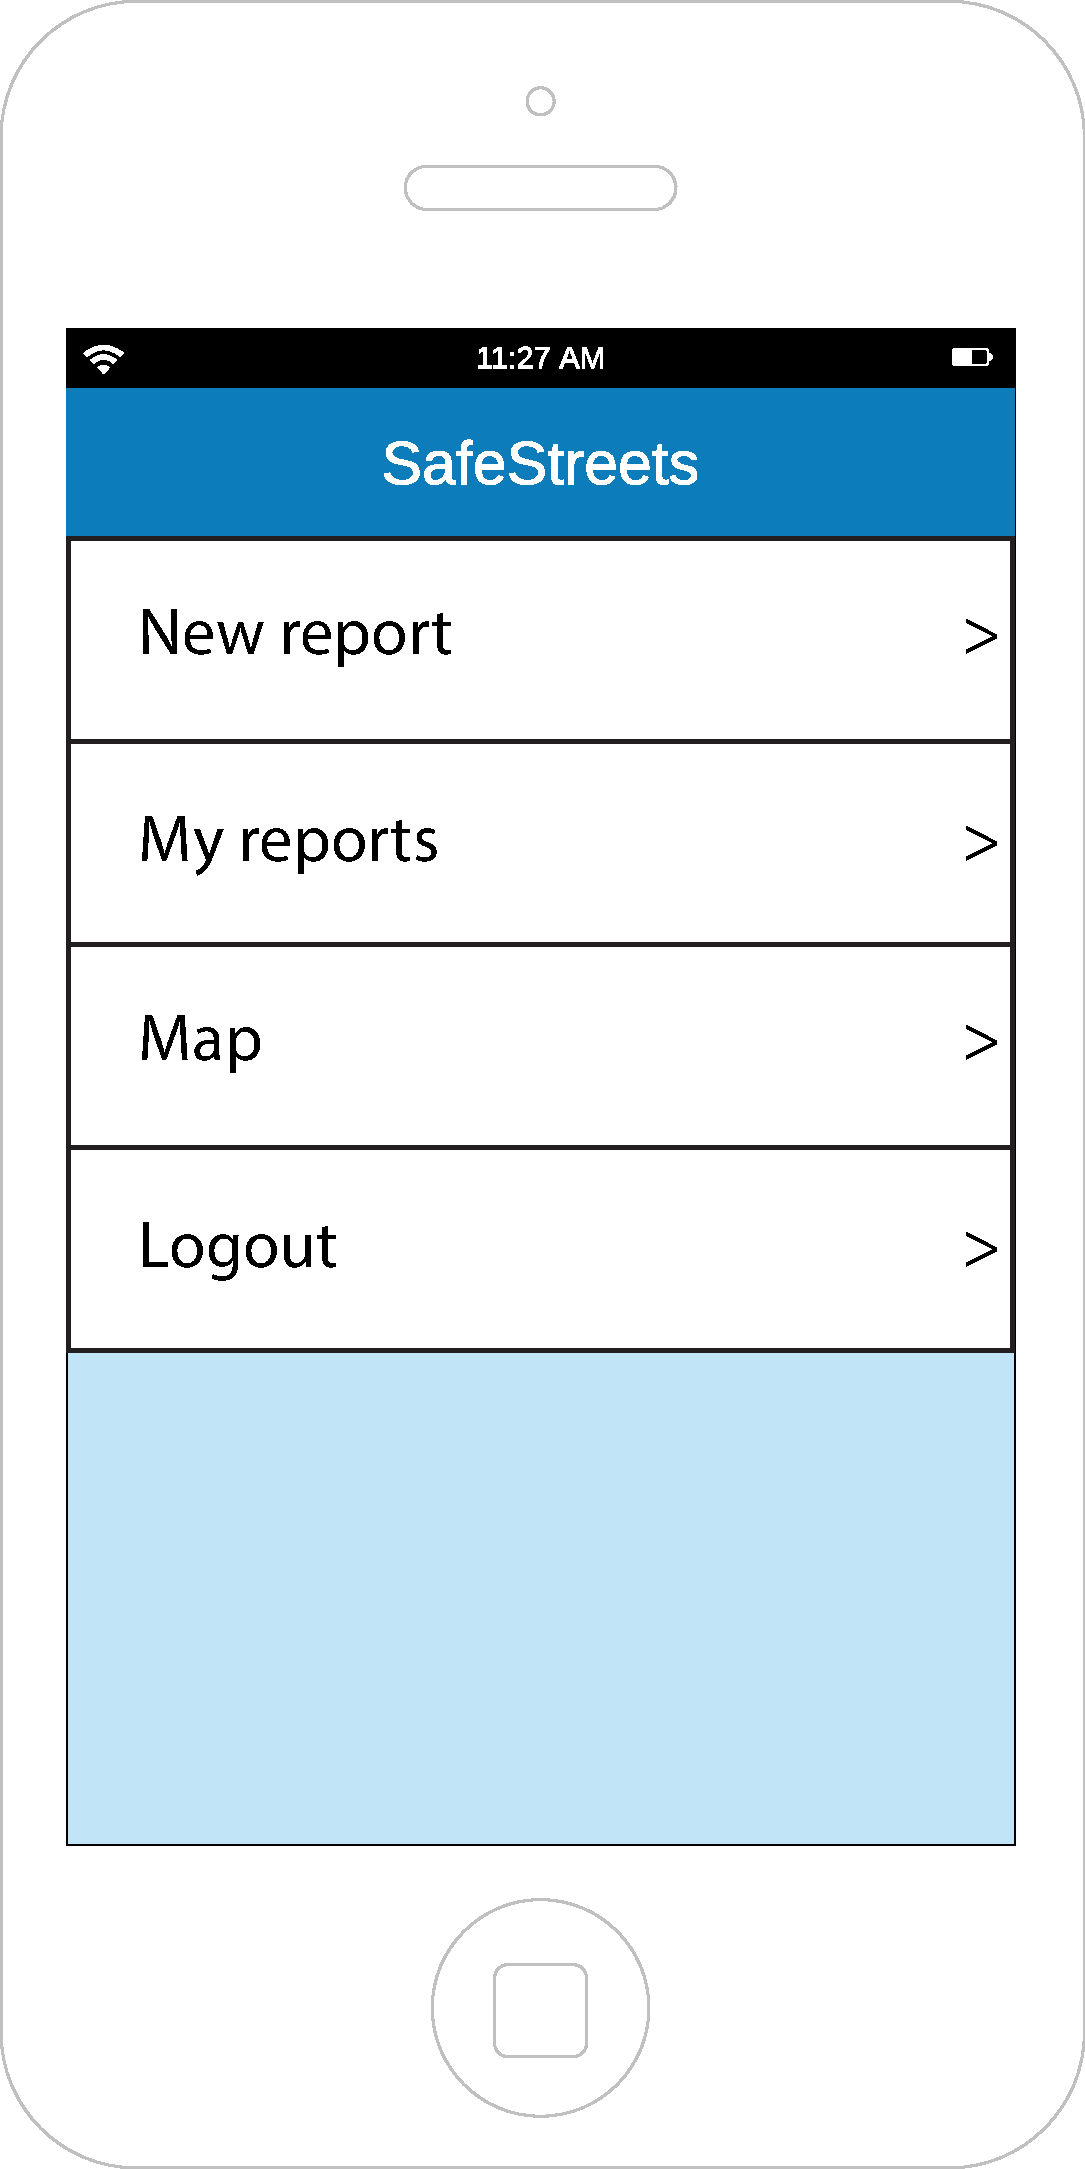
\includegraphics[scale=0.25, center]{Home}
			\caption{Home}
			\label{Home}
		\end{subfigure}
		\end{figure}

		\begin{figure}
		\begin{subfigure}{0.5\textwidth}
		\setcounter{subfigure}{2}
			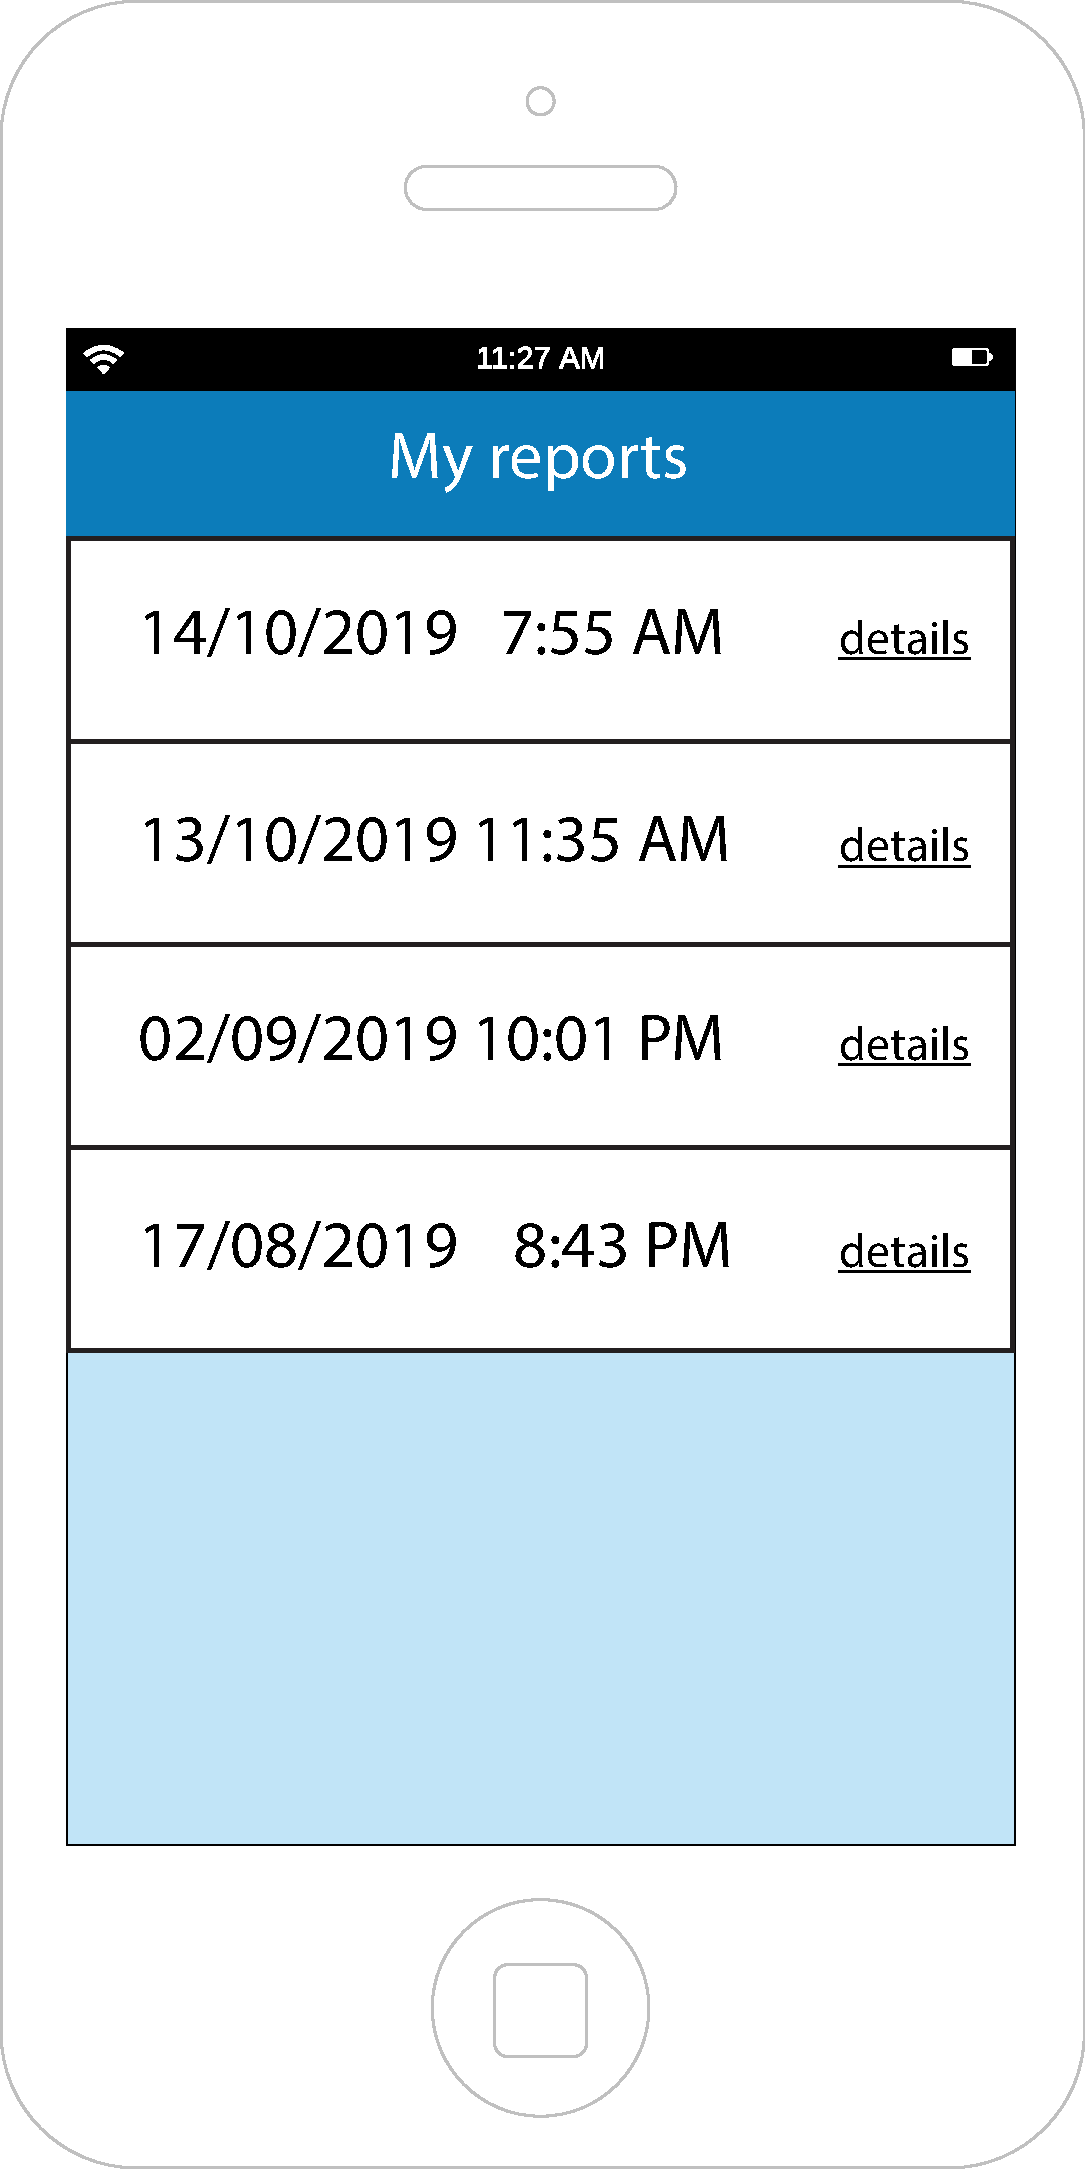
\includegraphics[scale=0.25, center]{Myreports}
			\caption{List of sent reports}
			\label{List of sent reports}
		\end{subfigure}
		\begin{subfigure}{0.5\textwidth}
			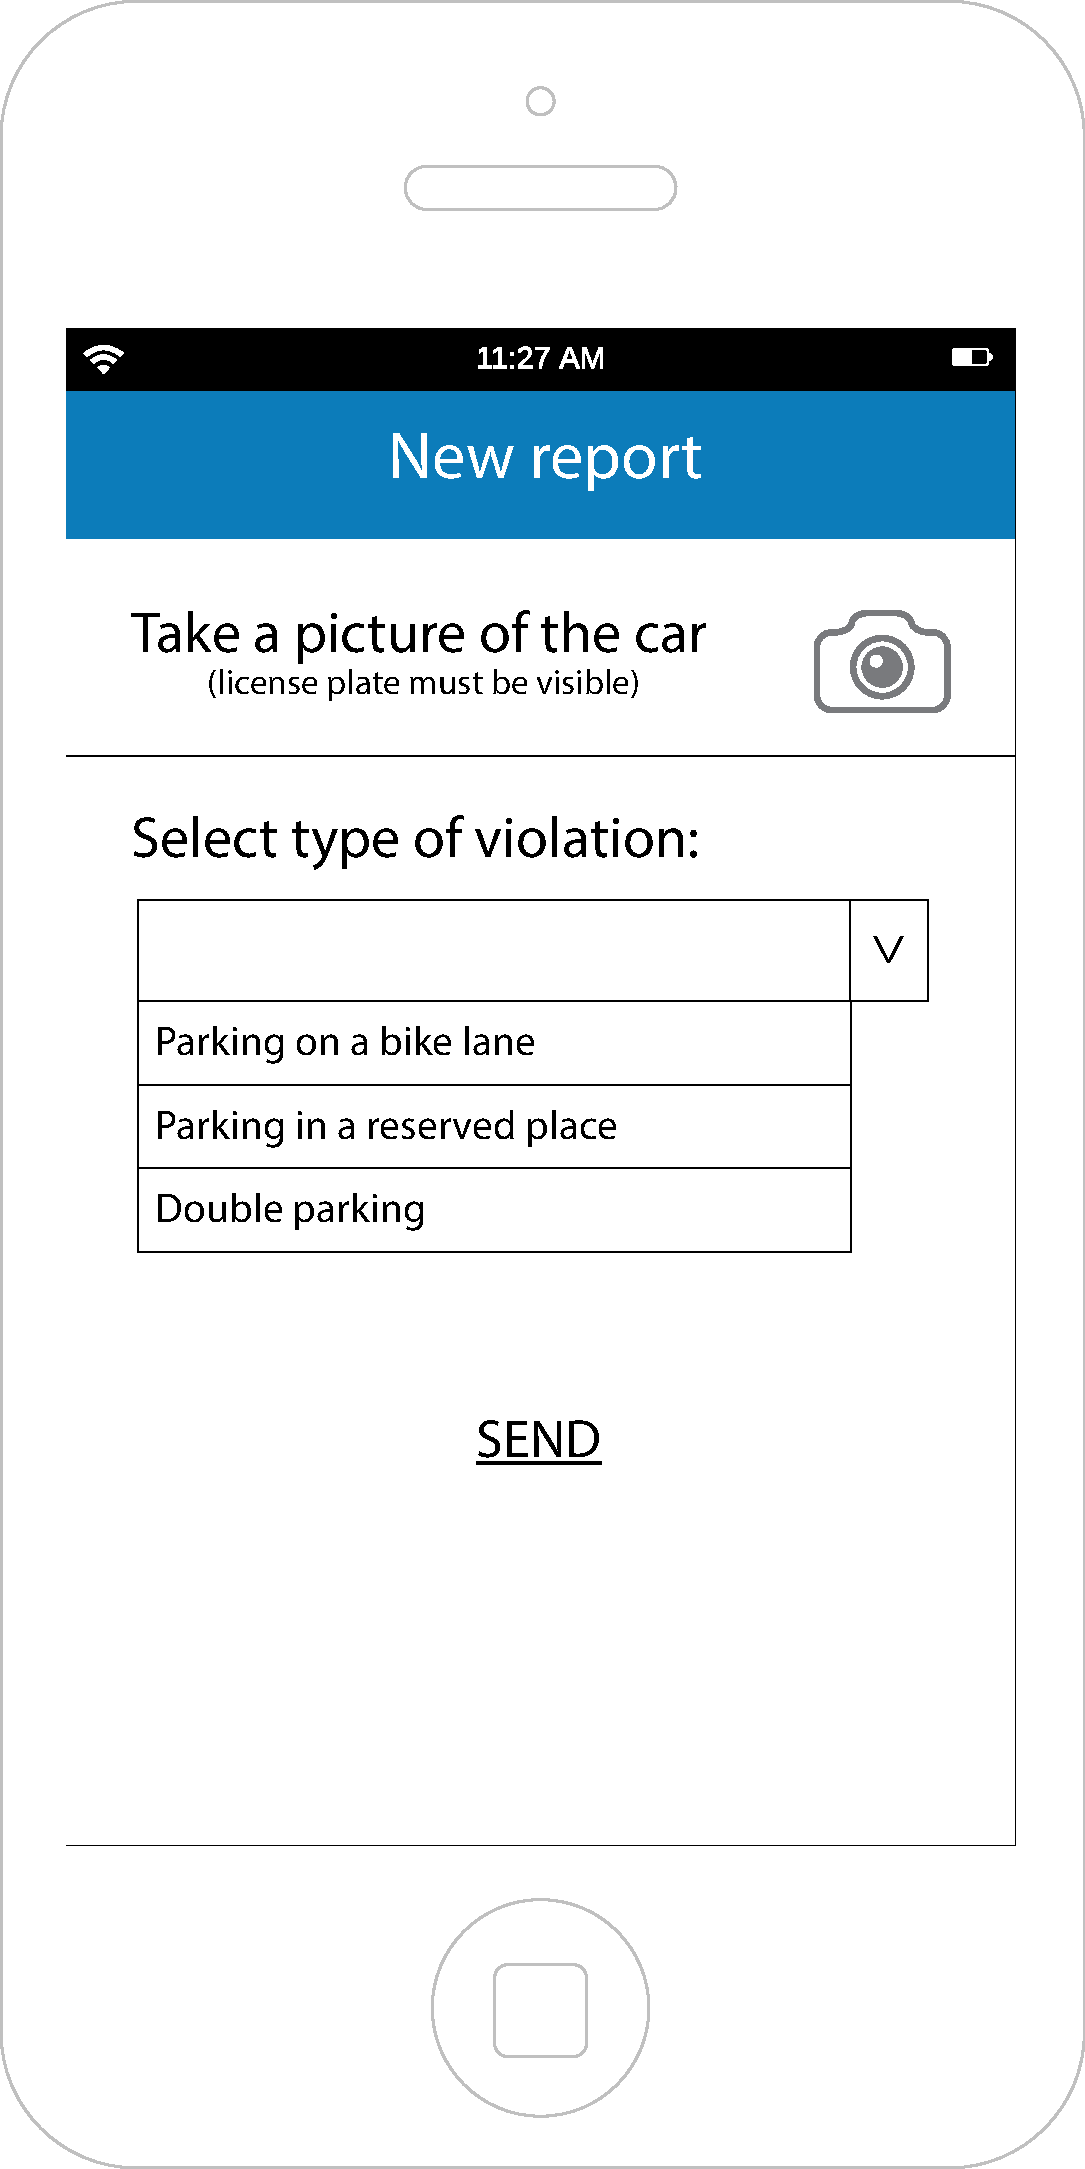
\includegraphics[scale=0.25, center]{Newreport}
			\caption{New report}
			\label{fig:subim2}
		\end{subfigure}
		\end{figure}
		\begin{figure}
		\begin{subfigure}{0.5\textwidth}
		\setcounter{subfigure}{4}
			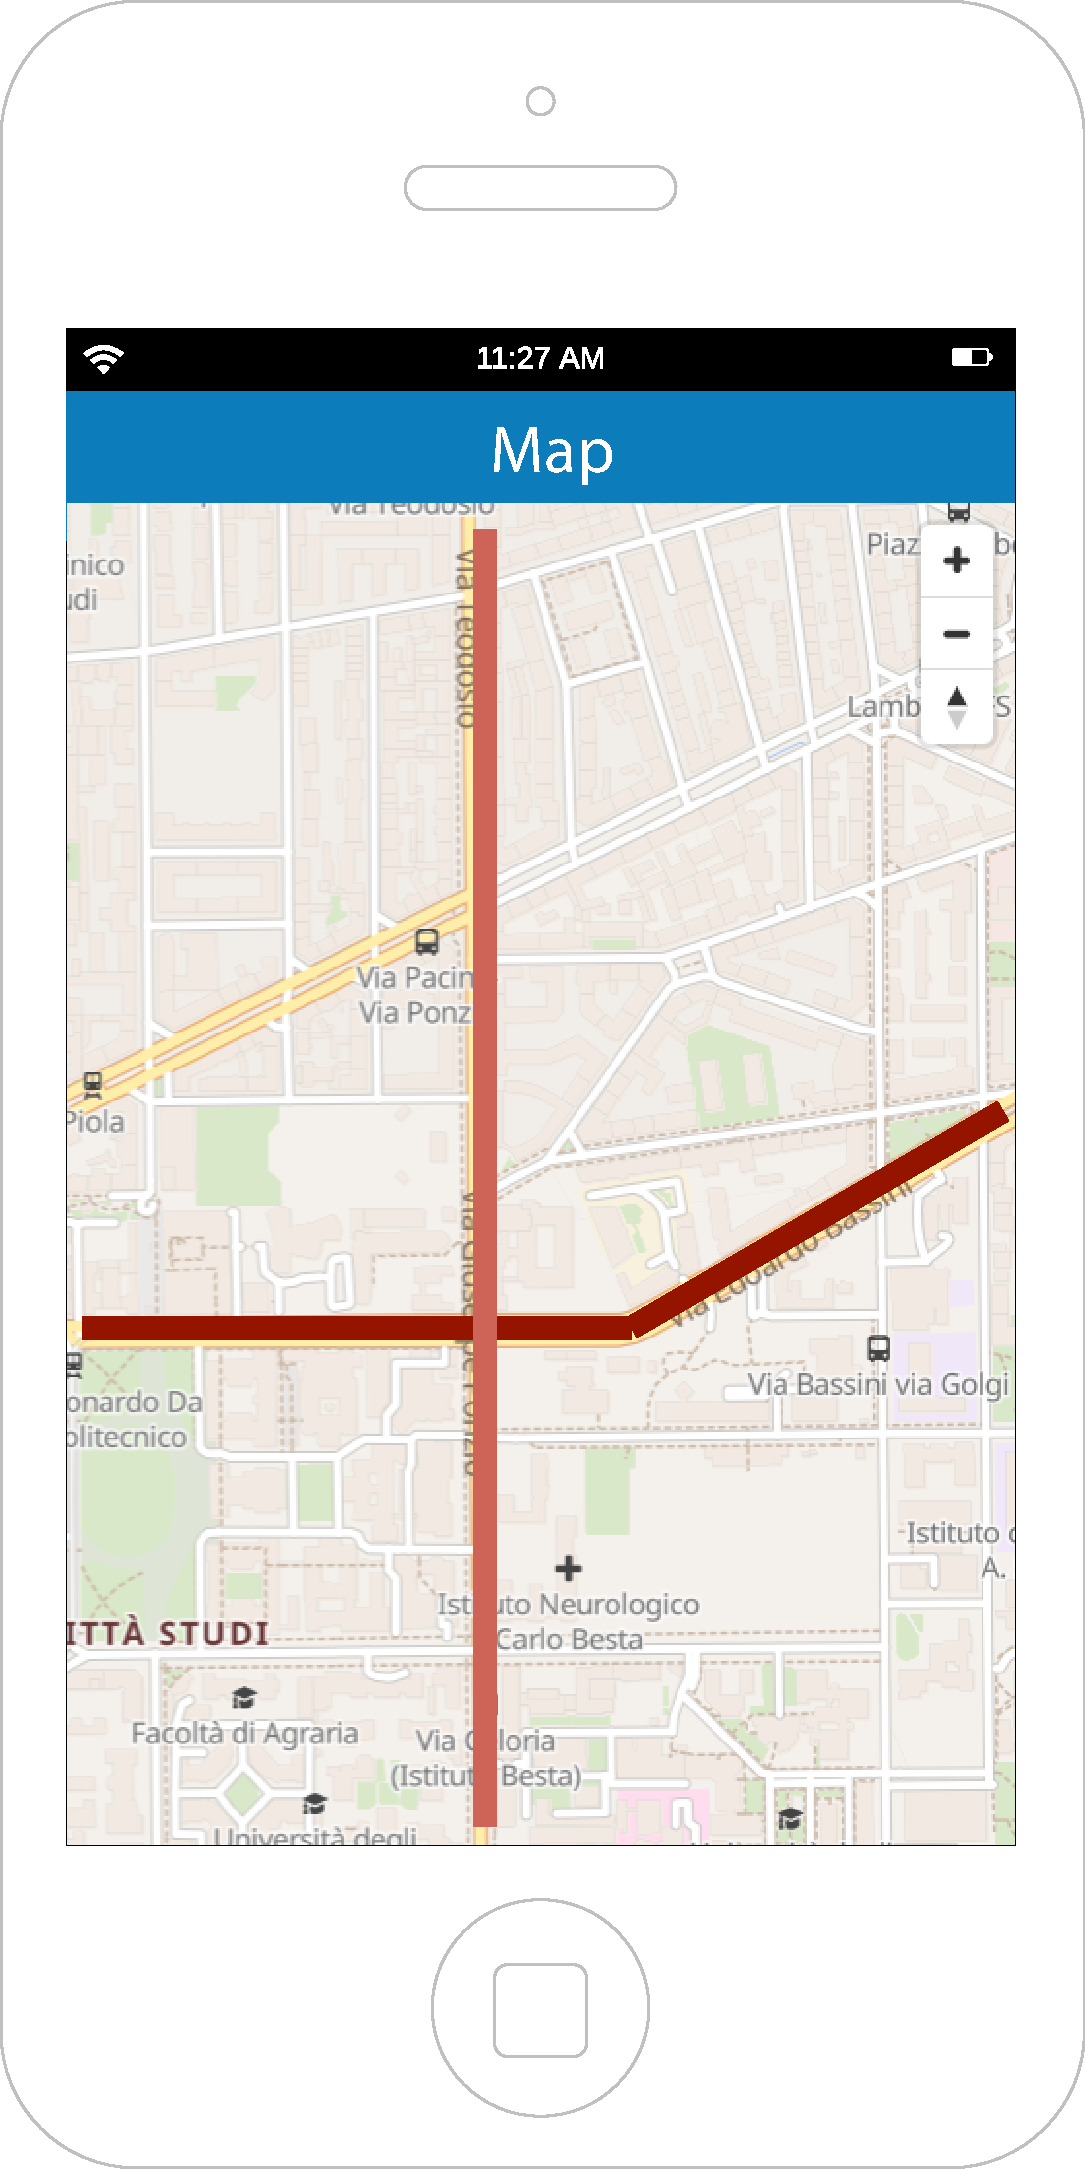
\includegraphics[scale=0.25, center]{Map}
			\caption{Map}
			\label{fig:subim2}
		\end{subfigure}
		\begin{subfigure}{0.5\textwidth}
			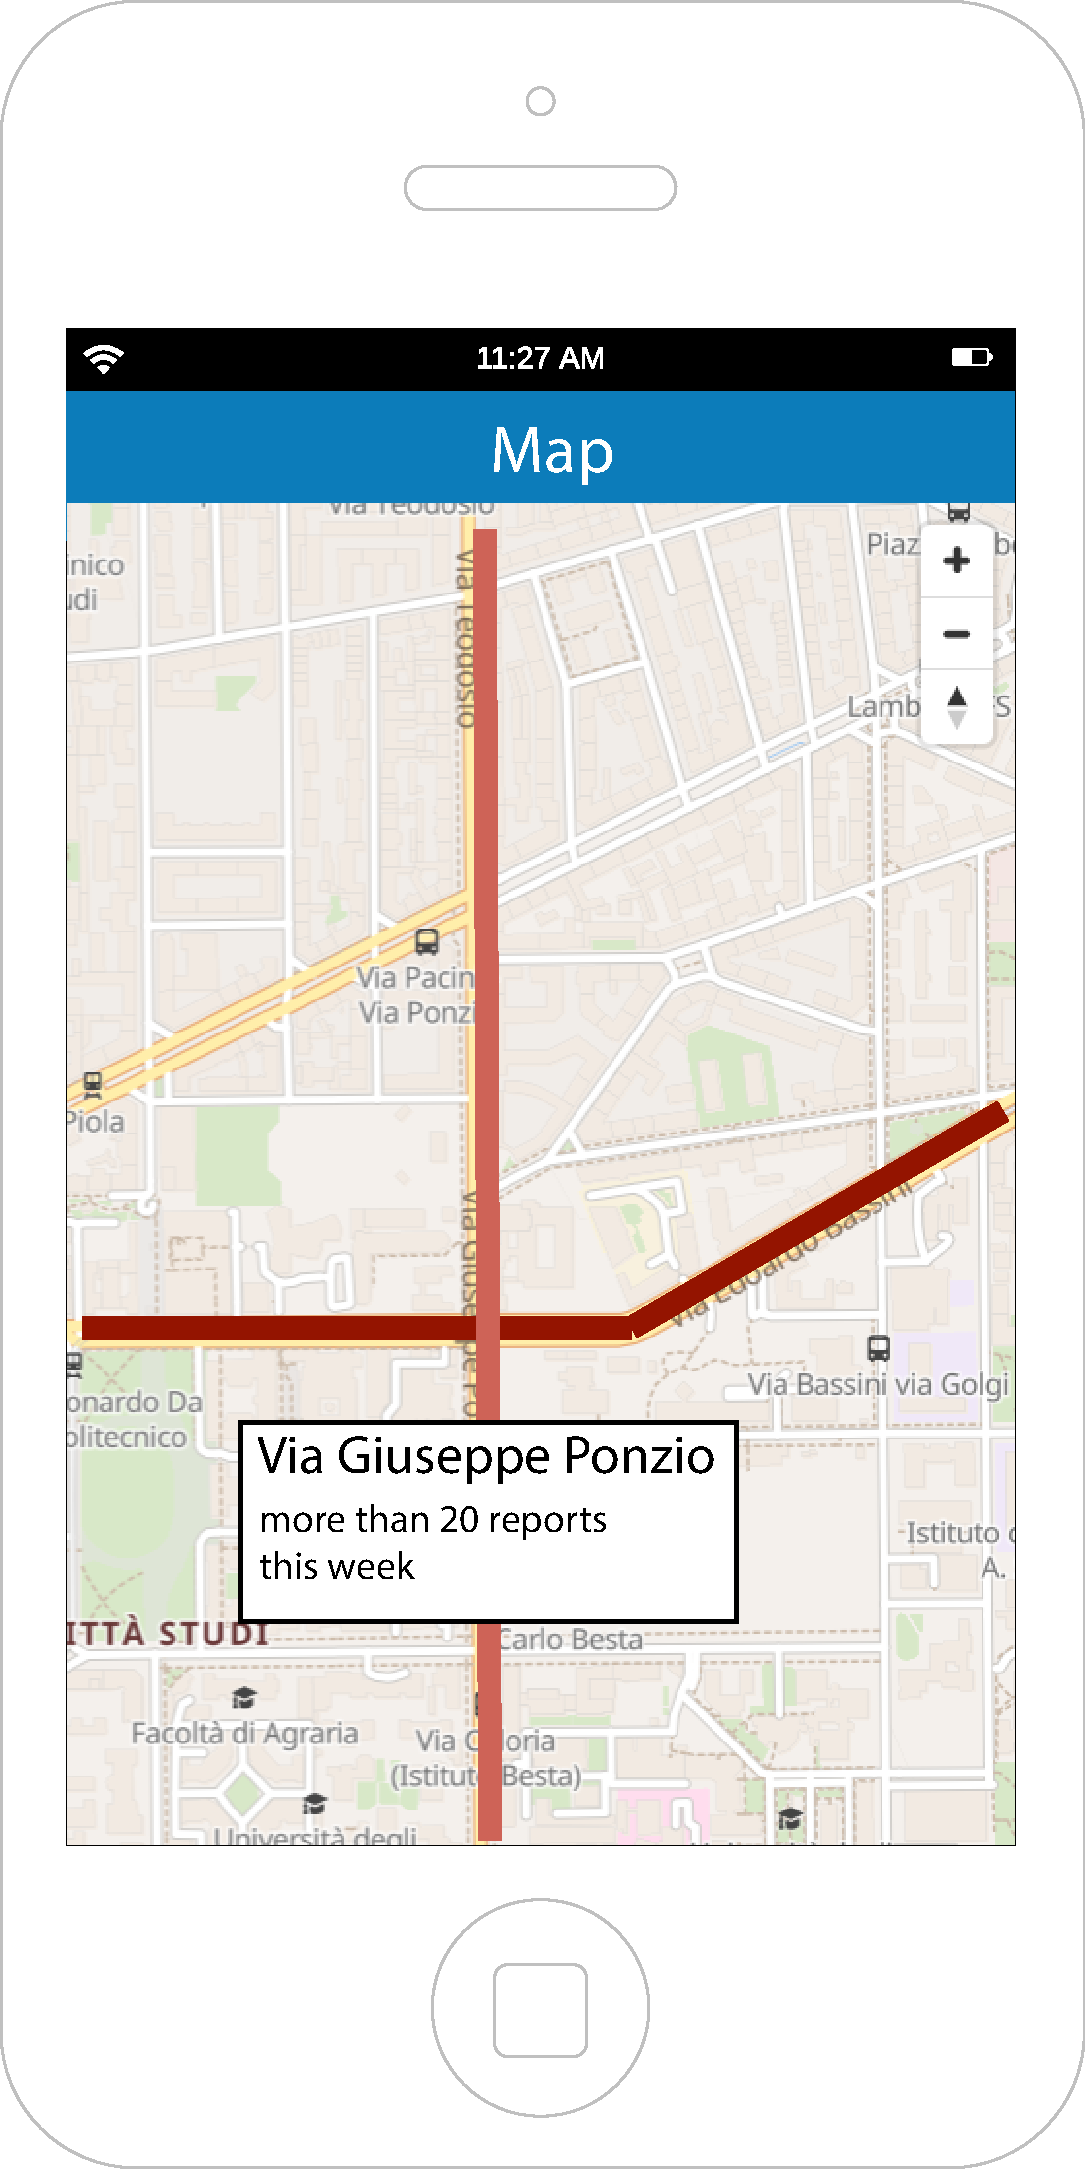
\includegraphics[scale=0.25, center]{Map-detail}
			\caption{Map - detail}
			\label{fig:subim2}
		\end{subfigure}
		\end{figure}

		\subsection{Hardware interfaces}
	The system has no hardware interfaces.
		\subsection{Software interfaces}
	The system has no software interfaces.
		\subsection{Communication interfaces}
	\section{Functional Requirements}
		\subsection{User}
			\paragraph{Scenario 1}
	
		\subsection{Authority}
	\section{Performances Requirments}
	\section{Design constraints}
		\subsection{Standards compliance}
		\subsection{Hardware limitations}
		\subsection{Any other costraint}
	\section{Software System Attributes}
		\subsection{Reliability}
		\subsection{Availability}
		\subsection{Security}
		\subsection{Maintainability}
		\subsection{Portablity}
% End of third chapter

\chapter{Formal Analysis}
% End of fourth chapter

\chapter{Effort Spent}
%End of fifth chapter

\chapter{References}
% End of sixth chapter

\end{document}